

\newpage
\section{Design and Implementation} \label{sec:dai}
This section will be discussing the main contribution of this project: a implementation of lattice Boltzmann method on SpiNNaker.  \\

All the source code is available at: \cite{spinn_lb}
\subsection{Implementation Overview}

As we discussed at \ref{sec:sdw}, in general, SpiNNaker development workflow, the first thing we did is to define the computation graph in Python. We will discuss how we define the lattice vertex (\ref{sec:tlc}), how we define our edge (\ref{sec:tle}), and how we connect them together as a graph (\ref{sec:tcg}). All these steps are implemented in the Python API.
1       
Then on the computation side, as discussed at \ref{sec:lbmb}, there are five steps for a lattice Boltzmann method in general. While the first four steps do not involve communication and can be calculated locally for each lattice vertex (discussed at \ref{sec:cp}), the last step, the streaming step, is where the communication happens, which we will focus on at \ref{sec:ssc}. These computation-wise codes are written in C.

\subsection{The Lattice Cell} \label{sec:tlc}
In this subsection, we will discuss how we design and implement the most basic component with the SpiNNaker GraphFrontEnd, the lattice basic cell.
\subsubsection{Design Consideration} \label{sec:tlcdc}
In the lattice cell class, we will define the data regions needed for simulation. In the implementation, it needs to acquire those data, reserve memory for the data and pass the data in SpiNNaker SDRAM in Python, then define how to read the data from the SDRAM during simulation in C. The data regions that a lattice might need for simulation are: \\

\begin{itemize}
    \item \textbf{System Information:} for every simulation, they at least need some memory reserved for the runtime system such as the how long is a machine time step. And the developers need to generate the system data region and allocate memory for them manually.
    
    \item \textbf{Transmission Information:} for non-embarrassingly parallel problems, the simulation is involved in communication. The keys are generated at runtime, and the developers can ask the mapping system for a fixed number of keys for every lattice. Then the mapping system would allocate continuous keys for the lattice, and the developers would get the base keys of them. The developers can apply for memory for the transmission keys and pass the keys to the cores, correspondingly.

    \item \textbf{Position Information:} in lattice Boltzmann, a lattice might need to know what is its position \textbf{(x,y)} among the whole simulation lattices. The position information would be generated when connecting the lattices as a graph and then pass them into the application.
    
    \item \textbf{Initialized Velocity:} in lattice Boltzmann method, the velocity needs to be generated according to the specific problem. We can either initialize it in Python then pass then in or initialize it in the simulation according to the position. A more detailed discussion is at \ref{sec:ip}.
    
    \item \textbf{Routing Information of Neighbours:} in lattice Boltzmann method, the lattice need to exchange the momentum and energy by moving the distribution function with its eight neighbours. This involves a few communication and the lattice need to know which are its eight neighbours and their routing information, i.e. routing keys to communicate with them. Thus allocating memory and pass them into the cores is necessary. 
    
    \item \textbf{Index of this Lattice:} we might need to know the index of the lattice in the whole simulation fabric. This might not be necessary for a simple prototype. The index of the lattice can be used as a timer delay to avoid communication traffic. We will discuss the communication at \ref{sec:ssc}.
    
    \item \textbf{Result Recording:} the SDRAM in SpiNNaker is relatively limited (\ref{sec:sa}). We can use the recorded data to store larger simulation result more reliably. We can tell the tools how much data per time step and the tools will determine the configuration to keep the SDRAM usage optimal.
\end{itemize}

\subsubsection{Final Implementation}
In the final implementation, we defined the discussed data regions in the \textit{LatticeBasicCell} class following the pattern: get the data; allocate memory; write the data in, where the first step is defined by the developer and the latter two steps are written in Python scripts, and the tool will interpret the scripts to do the actual work. For different data, there are different way to get the data:

\begin{itemize}
    \item \textbf{System Information:} the \textit{SpiNNaker GraphFrontEnd} provide API to generate the system data region.
    \item \textbf{Transmission Information:} the SpiNNaker runtime would allocate keys for the cores.
    \item \textbf{Position Information:} the position information is decided during runtime. it will be passed as class variables.
    \item \textbf{Initialized Velocity:} the velocities are decided during runtime with an initialization function. They will be passed as class variables. 
    \item \textbf{Routing Information of Neighbours:} a lattice can know the which are its neighbours by asking the connected edges. We will illustrate how we implement it at \ref{sec:tle}. After knowing its neighbours, we can get their routing keys via the get\_routing\_info\_from\_pre\_vertex() function from the \textbf{PACMAN} library.
    \item \textbf{Index of Lattice:} we can ask the graph system for the index of a lattice.
    \item \textbf{Result Recording:} we do not need to get data from result recording since it is for the result.
\end{itemize}

After all the data are acquired, we get then reserve corresponding memory and write the data into the SDRAM of each SpiNNaker core; see the upper part of Fig.~\ref{fig:write_data}. Correspondingly, in the C file, we also need to read the data from the SDRAM before the simulation; see the bottom part of Fig.\ref{fig:write_data}. The Fig.~\ref{fig:write_data} shows how we reserve memory for the different data regions and write the data into the SDRAM followed by how to read the written data from the SDRAM during runtime in C.\\
\begin{figure}[tb]
   \centering
       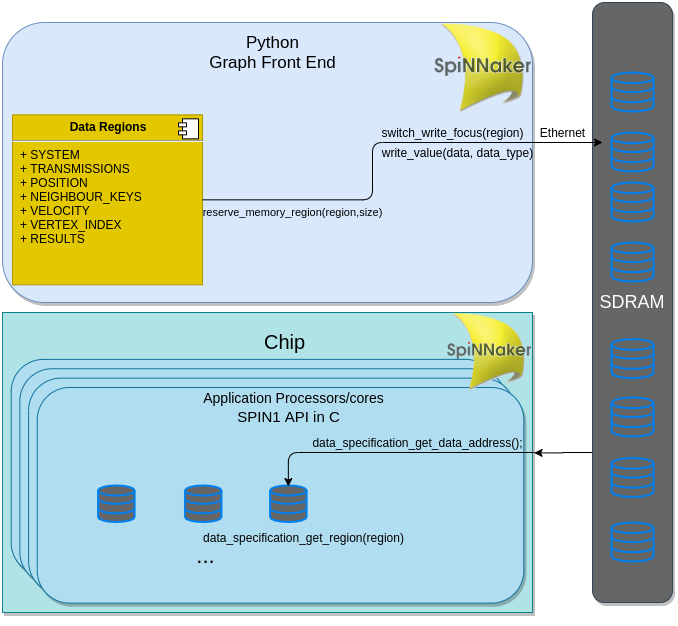
\includegraphics[width=1\textwidth]{figures/write_data.png}
       \caption{A lattice cell A connected by another lattice B via a lattice edge with the compass being "W". The lattice A then can get the routing key from its pre\_vertex, B.}
       \label{fig:write_data}
\end{figure}



\subsection{The Lattice Edge} \label{sec:tle}
\subsubsection{Design Consideration}
The major job of the lattice edge except connecting two lattice cells is providing a way that the lattice cell can get the vertex on the other end of this edge in a given direction. So that each lattice can get the routing information (routing keys) of its eight neighbours with knowing the direction. \\
\subsubsection{Final Implementation}
In the implementation, the \textit{Lattice Edge class} inherit from the \textit{MachineEdge}, which provided a way to record the pre-vertex and post-vertex, from the \textbf{PACMAN} library. Then we introduced another attribute, \textbf{compass}, to record the relative position of the pre-vertex; see Fig.~\ref{fig:edge}.\\
\begin{figure}[tb]
   \centering
       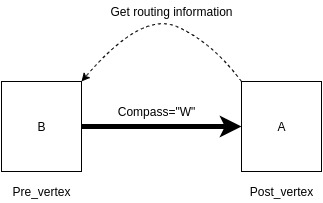
\includegraphics[width=0.7\textwidth]{figures/edge.jpg}
       \caption{A lattice cell A connected by another lattice B via a lattice edge with the compass being "W". The lattice A then can get the routing key from its pre\_vertex, B.}
       \label{fig:edge}
\end{figure}

\subsection{The Computational Graph} \label{sec:tcg} 
\subsubsection{Design Consideration}
In the selected test problem from Minion and Brown\cite{minion1997performance}, the boundary condition we applied for this project is a periodic condition. In the C implementation, we implemented the periodic condition is halo-swapping; see Fig.~\ref{fig:haloswap}. The periodic condition is explicitly applied to the post-collision distribution function $f_i^{*}$ in the streaming step, which introduced extra memory consumption and complexity into the development.\\

Fortunately, in SpiNNaker, the developers do not implement the halo-swapping to apply to the periodic condition explicitly. Instead, SpiNNaker developers can simply connect the lattices on one fringe to the lattices on the opposite fringe via the implemented \textit{Lattice Edge}; see Fig.~\ref{fig:spinnaker_halo}.\\


\begin{figure}[htbp]

\begin{subfigure}[b]{1\textwidth}
       \centering
       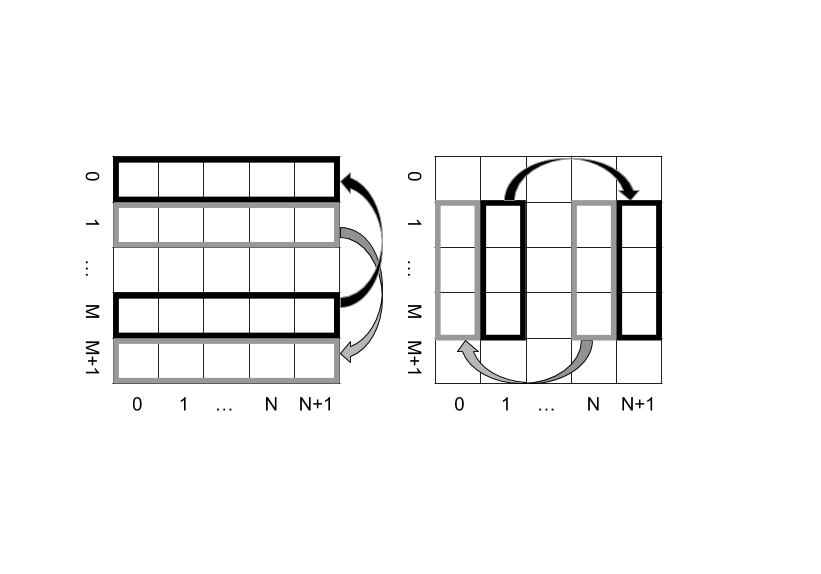
\includegraphics[width=0.8\textwidth]{figures/haloswap.png}
       \caption{A periodic condition in M$\times$N lattice Boltzmann implemented by halo-swapping. We apply this method in our serial C implementation.}
       \label{fig:haloswap}
   \end{subfigure}
   \begin{subfigure}[b]{1\textwidth}
       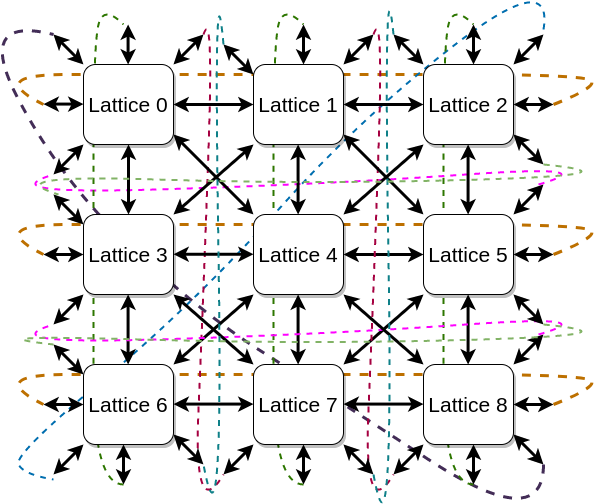
\includegraphics[width=\textwidth]{figures/2dfabric.png}
       \caption{A periodic condition in 3$\times$3 lattice Boltzmann implemented by connecting the lattice periodically via lattice edge. We apply this method in the SpiNNaker implementation.}
       \label{fig:spinnaker_halo}
   \end{subfigure}
   \caption{How we implement a periodic condition in C (\ref{fig:haloswap}) via halo-swap and in SpiNNaker (\ref{fig:spinnaker_halo}) via SpiNNaker graph edge.}
\end{figure}

\subsubsection{Final Implementation}
As we designed, to implement a periodic condition, we connect the lattice cells periodically via lattice edge; see Algo.~\ref{algo:periodic}.\\

\begin{algorithm}
 \caption{The Algorithm to connect the lattice with a periodic condition}
 \label{algo:periodic}
 \KwData{Scale in x dimension: X; Scale in y dimension: Y}
 \SetKwFunction{Connect:}{connect two lattice via a lattice edge}
 \For{i in 0...X}{
    \For {j in 0...Y} {
       Connect Lattice(i,j) with Lattice(i,(j + 1) mod Y)\;
       Connect Lattice(i,j) with Lattice((i + 1) mod X,(j + 1) mod Y)\;
       Connect Lattice(i,j) with Lattice((i+1) mod X, j)\;
       Connect Lattice(i,j) with Lattice((i+1) mod X, (j-1) mod Y)\;
       Connect Lattice(i,j) with Lattice(i, (j-1) mod Y)\;
       Connect Lattice(i,j) with Lattice((i-1) mod X, (j-1) mod Y)\;
       Connect Lattice(i,j) with Lattice((i-1) mod X, j)\;
       Connect Lattice(i,j) with Lattice((i-1) mod X,  (j+1) mod Y)\;
    }
 }
\end{algorithm}




\subsection{Initialize Parameters} \label{sec:ip}
In this subsection, we will discuss how we consider the two different ways to initialize parameters, how we decide and how we implement.\\
\subsubsection{Design Consideration}
To initialize the parameters for the lattice Boltzmann, there are two different ways in general. The first one is initialization on the host (in Python) then passing the initialized parameters into the simulation, and the other one is initialization on SpiNNaker (in C).\\

When initializing parameters in Python on the host, we need to compute the parameters in serial nested loops before the SpiNNaker actually run the simulation. On contrast. If we are initializing the parameters in SpiNNaker, the parameters would be computed distributively on each individual core. Besides, vanilla Python is commonly regarded as being poor in scientific computing, especially in nested loop.\\

It is reasonable that initialization in C on the simulation runtime would be faster in speed comparing with initialization in Python in serial. Thus, our first implementation was based on C and computed the initial parameters distributively on each core. \\

However, there are two points that we do not take into consideration when it comes to the real implementation on SpiNNaker. The first one is that, as we introduced before \ref{sec:ca}, SpiNNaker is using ARM968 cores which have no floating-point hardware, and we have to use fixed-point arithmetic or software-based floating-point arithmetic. It introduced some challenges in using the mathematical library in C, including \textbf{math.h}. The other one is that, as we also introduced before \ref{sec:ca}, the SpiNNaker cores have relatively limited ITCM (instruction tight-coupled memory). If we use the mathematical library such as \textbf{math.h}, the bloated math library will run out of the limited ITCM. Although it is possible to implement mathematics functions such as \textbf{tanh} by applying the Taylor series, the accuracy and efficiency of the hand-write functions do not satisfy the requirements of this simulation.\\

After carefully reconsidering the whole process, we finally decided to implement the initialization on the host in Python and then write the initialized parameters as data regions into the SpiNNaker device. \\
\subsubsection{Final Implementation}
we had implemented the initialization function in C for the serial version; see Appendix.~\ref{app:a}. It uses two-level nested-loop to initialize the velocities and the macroscopic densities for every actual lattice according to the settings of the test problem. Here the actual lattices are those which sit in the inner part of the simulation and the outermost layer would be used as halo-swapping.\\

For SpiNNaker version, since we have to instantiate the LatticeBasicCell class and the initialized parameters need to be passed as attributes during the instantiation, instead of calculating the parameters of all lattices at once, we calculate the parameters every time before a lattice being created. Then when the lattices are created, the parameters are initialized as well.\\

In the implementation of the SpiNNaker version of LBM, we implement the initialization of velocity function in Python and pass the result as attributes before the instantiation. For the macroscopic density, since we are setting all the initial macroscopic densities $\rho$ as 1.0, we can directly initialize them in the C source file.  \\

\subsection{Computation Implementation} \label{sec:cp}
This subsection will discuss how we design and implement the behaviours except inter-core communication of a lattice.\\
\subsubsection{Design Consideration}
The computation part of the simulation is the process that does not involve communication. According to the five steps of a lattice Boltzmann method in \ref{sec:lbmb}, we can draw the algorithm for each individual lattice; see Algo.~\ref{algo:lbm}.\\

\begin{algorithm}
 \caption{The Algorithm of the lattice Boltzmann method for a individual lattice.}
 \label{algo:lbm}
 Initialize\;
 \While {not finish} {
  compute $\rho$ and $\vec u$\;
 compute $f_i^{eq}$\;
 \tcc{Collision Step}
 collideStep: Move $f_i$ to $f^*$ \;  
  \tcc {Streaming step start}
 Send $f_i$ to its neighbours\;  
 Receive neighbours' $f_i$ as $f_i^{*}$\; 
 \tcc {Streaming step end}
 }
 
\end{algorithm}

From the Algo.~\ref{algo:lbm}, we can see that the algorithm except the streaming steps do not need any inter-core communication, and those computations can be done distributively by each individual core.\\

\subsubsection{Final Implementation}
For the actual implementation, we need to take SpiNNaker's features into account. In this project, we use the time ticker provided by SpiNNaker as a trigger for each iteration instead of directly execute the loops. The reason why we choose this method is that it provides an easier way to manage the communication, which we will discuss in \ref{sec:co}.\\

\begin{figure}[!tb]
   \centering
       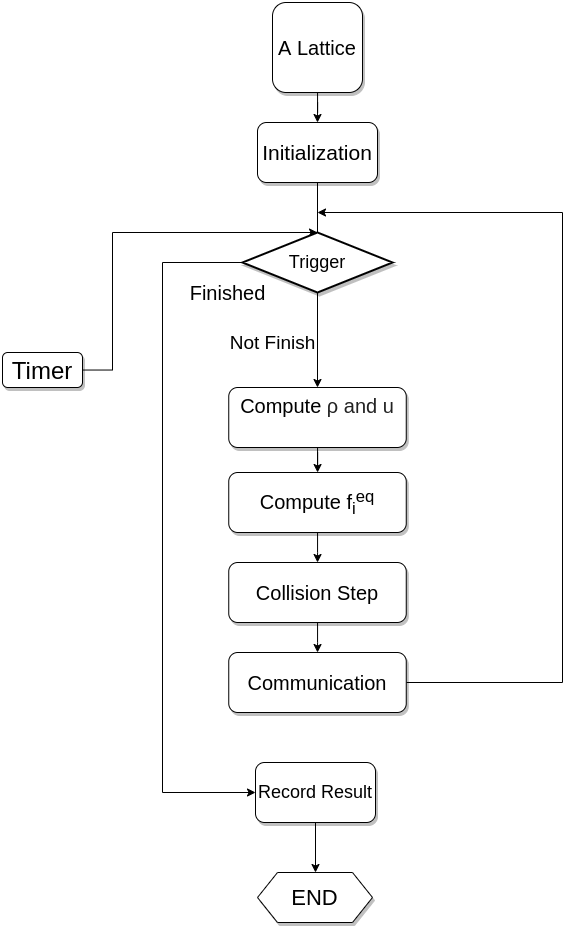
\includegraphics[width=0.6\textwidth]{figures/computation.png}
       \caption{A diagram of the computation processes of a Lattice. After initialization, the lattice starts the simulation. The built-in timer will send a timer tick for every a fixed time, and the time tick would trigger the simulation for the next time step until the simulation ends. In this case, we do not take the communication into consideration.}
       \label{fig:computation}
\end{figure}

As Fig.~\ref{fig:computation} shows, the after the initialization, whenever the lattice receive a time tick and the simulation is not ending, it will run another computation loop. After all, simulations completed at this core, it will record the result to the buffer and change its state as ready for the front end extracting the buffer.\\

\subsection{Communication Implementation} \label{sec:ssc}
As we discussed above, the only part of LBM that involve communication is the streaming step. Therefore, in this subsection, we will discuss how we design the steaming step of the lattice and how we implement sending the multicast packets and acquired the data.\\
\subsubsection{Design Consideration}
Firstly, we need to consider what data we need to seed via multicast. In the steaming step of the lattice Boltzmann method, the post-distribution functions $f_i^*$ in nine directions are the distribution function of its neighbours in the corresponding directions. In this case, for each individual lattice, since it is itself in the first direction, it need to send its rest eight distribution functions $f_i$ via multicast; see Fig.~\ref{fig:spinn_send}. In this case, the number of multicast packets is 8.\\

Then we have to consider the multicast packets each lattice need. As we discussed above, each lattice will send eight multicast packets from each of its neighbours. Therefore, the total multicast packets a lattice need to acquire is $8 \times 8 = 64$; see Fig.~\ref{fig:spinn_receive}.\\

\begin{figure}[!tb]

\begin{subfigure}[!tb]{0.5\textwidth}
       \centering
       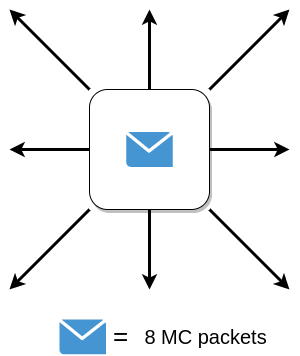
\includegraphics[width=0.5\textwidth]{figures/send.png}
       \caption{A lattice send its distribution function $f_i$ in 8 directions via SpiNNaker multicast. For every streaming step, the lattice will send 8 multicast packets.}
       \label{fig:spinn_send}
   \end{subfigure}
   \begin{subfigure}[!tb]{0.5\textwidth}
   \centering
       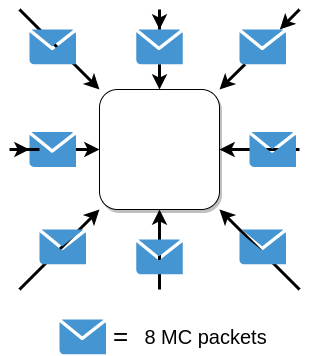
\includegraphics[width=0.5\textwidth]{figures/receive.png}
       \caption{A lattice acquire the distribution function of its 8 neighbours from multicast packets as it post distribution function $f_i^{*}$. For every streaming step, the lattice will receive $8\times8=64$ packets.}
       \label{fig:spinn_receive}
   \end{subfigure}
   \caption{How a lattice send it distribution function $f_i$ (\ref{fig:spinn_send}) and hot it acquire the post distribution function ($f_i^{*}$) from the arriving multicast packets from its neighbours (\ref{fig:spinn_receive}).}
\end{figure}

However, not all 64 multicast packets are necessary for a lattice. From each direction, the lattice only needs the corresponding one distribution function. In other words, the lattice only needs one multicast packet from one direction. Therefore, a lattice only actually need eight multicast packets though it still needs to acquire all 64 packets to know which are eight packets it needs.\\

\subsubsection{Implementation}
In the implementation, the first challenge is that, in SpiNNaker, by default, we can only send 32bit integer via multicast packet, while the numerical format we used in this project is floating-point. Our solution, which is also the commonly used solution in SpiNNaker, is converting the floating-point number to unsigned integer when sending the multicast packets and convert the unsigned integer back to floating-point when reading the payload of multicast packets by using the \textbf{union} structure in C.\\

The second challenge is to recognize where a packet comes from. In the implementation, instead of only adding the payloads of the packets, we add both the key and the payload into the circular buffer. Then we can firstly get the key of the packet knowing the packet coming from which direction then get the corresponding payload.\\

Finally, because SpiNNaker multicast does not guarantee the delivery of packets, to ensure that every lattice receives the correct number of packets, we implement a safety check function to interrupt the program when not all lattice receive the correct number of multicast packets. As we discussed before, for every time step, each lattice should receive 64 packets, where 8 of them is necessary, and 56 of them should also be confirmed as delivered for the sake of safety.\\

In conclusion, as Fig.~\ref{fig:communicate} shows, to implement the steaming step by communication, the lattice will first convert the corresponding distribution function from floating-point to unsigned integer. Then it sends the converted payload with the corresponding key. On the receiver side, it will first store both the key and payload into the circular buffer. When it collects the correct number of buffer (in this case, the correct number of the buffer is $64\times2 = 128$), it will extract key and payload from the buffer. Finally, the receiver will save the convert-backed payload into $f_i^*$ as post-distribution function and the streaming step end.\\
\begin{figure}[!tb]
   \centering
       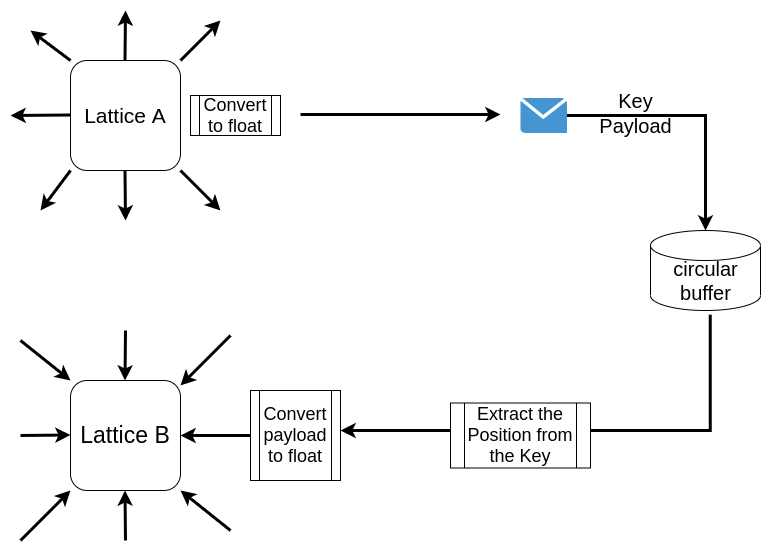
\includegraphics[width=0.8\textwidth]{figures/communication.png}
       \caption{A diagram of the communication process between two adjacent lattices. In this diagram, Lattice A sends a multicast packet, and Lattice B is one of the receivers. Before A sending the MC packets, it firstly converts the distribution function $f_i$ into an integer. Then it sends the converted $f_i$ with the corresponding key. When Lattice B captures the MC packet, it firstly adds the key and payload into the circular buffer. When B capture all the packets for this time step, it stores  the packets of them to $f_i^*$ as post-distribution function.}
       \label{fig:communicate}
\end{figure}

This report up to this point has described how to implement a basic lattice Boltzmann method on SpiNNaker, and it is sufficient for simulation in relatively small simulation (e.g. 32 lattices $\times$ 32 lattices). However, for real-world simulation, the scalability is important. We need to do further optimization for the potential real-world simulation.\\

\subsection{Communication Optimization} \label{sec:co}
In this section, we will first discuss why the basic implementation cannot run large scale simulation in a relatively short time. Then we will introduce how we optimize the communication for the potential larger simulation.\\
\subsubsection{Design Consideration}
As we illustrated before, because there is no guarantee of packet delivery and other issues including back pressure and packets collision will cause packets drop, we introduced a safety check before every time step. The simulation will always pass the safety check when there are only a small number of packets firing in the network when the scale of simulation is relatively small. However, if the simulation scale becomes larger enough, there would be more packets in the network during the same period of time. Although, if there is a dumped packet, the re-injector would have the ability to re-inject. When some unnecessary procedures slowing down the simulation and there are too many packets firing at the same time; see Fig.~\ref{fig:packet_error}, the re-injector might not be able to re-inject and, as a consequence, the simulation will not pass the safety check for the next time step. Eventually, the program would produce a runtime error.\\

\begin{figure}[!tb]
   \centering
       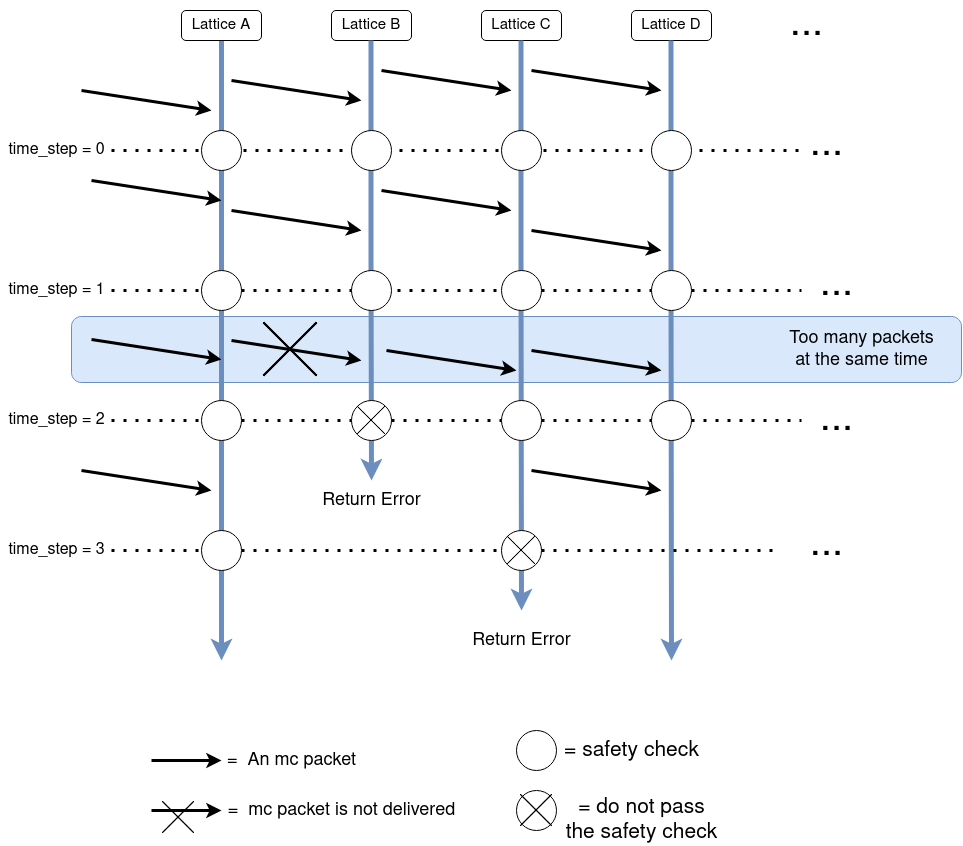
\includegraphics[width=1\textwidth]{figures/packet_error.png}
       \caption{When there are too many packets firing in the network at the same time, it is highly possible that the packets would be dumped. Though the re-injector might be able to re-inject the packets, when there are too many packets need to re-inject and the time is not enough, the lattice (lattice A in this diagram) will not pass the safety check and return a runtime error. The simulation of this core then will stop. The other core will stop because of safety check successively.}
       \label{fig:packet_error}
\end{figure}
\subsubsection{Final Implementation}
In order to address these issues, firstly we remove all unnecessary procedures, i.e. printing log information to the IO buffer and only remain those logs which are essential for debugging.\\

Secondly, to reduce the peak packet rate, we firstly introduced a delay between sending multicast packets. In the implementation, to make the delays of the lattices as different from each other as possible, we add delays based on the index of cores; see Fig.~\ref{fig:packet_offset}. With considering not introduce a too big delay when the scale of simulation is large, after experiments, we finally use Index mod $400$ as the delay between sending.\\

Finally, even though we have made some efforts to reduce the peak packet rate, for an even larger simulation, we need to reduce it even further. Therefore, we further introduce timer offset to further reduce the chance of them sending messages at the same time; see Fig.~\ref{fig:packet_offset}.\\

\begin{figure}[!tb]
   \centering
       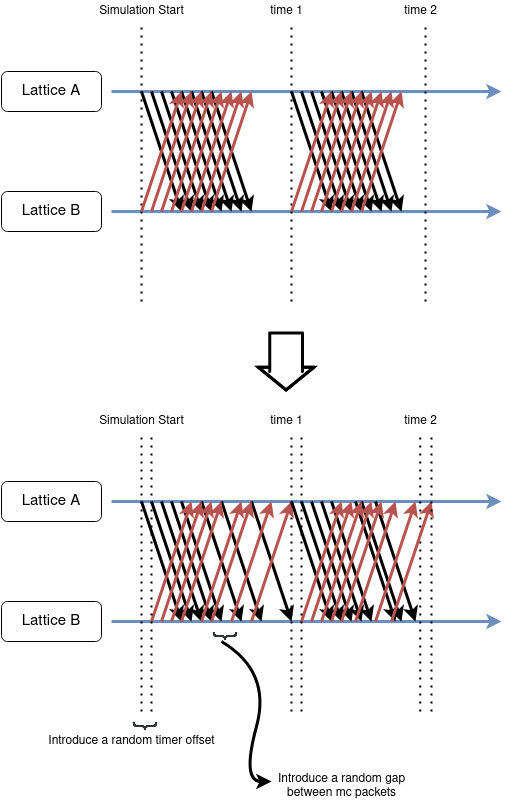
\includegraphics[width=0.8\textwidth]{figures/optimize.png}
       \caption{When there are too many packets firing in the network at the same time, it is highly possible that the packets would be dumped. Though the re-injector might be able to re-inject the packets, when there are too many packets need to re-inject and the time is not enough, the lattice (lattice A in this diagram) will not pass the safety check and return a runtime error. The simulation of this core then will stop. The other core will stop because of safety check successively.}
       \label{fig:packet_offset}
\end{figure}

